\documentclass[11pt, a4paper]{article}
\usepackage[spanish]{babel}
\usepackage{geometry}
\usepackage{graphicx}
\usepackage{amsmath, amssymb}
\usepackage{xcolor}


\geometry{
	left=2.5cm,
	right=2.5cm,
	top=3cm,
	bottom=3cm
}

\pagestyle{plain}

%opening
\title{Obligatorio 2 \\ Cálculo en una variable}
\author{Juan Pablo Canedo y Franco Cardozo}
\date{}

\begin{document}

\maketitle
\clearpage

\section{Parte 1: Consumo energético}

$$C(t) = 2 + 3 \sin^2 \left(\frac{\pi t}{12}\right)$$


\subsection{Interpreta el significado físico de la función $C(t)$.}
La constante 2 indica que el consumo mínimo de energía será de 2 kW, mientras que $(3 \sin^2 \left(\frac{\pi t}{12}\right))$ modela la variación de consumo en cada momento a lo largo de un día.

\subsection{ Calcula el consumo total de energía entre las 0 y las 24 horas usando una integral definida.}

\begin{align*}
    & \int_{0}^{24} \left(2 + 3\sin^2\left(\frac{\pi t}{12}\right)\right) dt \\
    &= \int_{0}^{24} 2 \, dt \quad + \quad \int_{0}^{24} 3\sin^2\left(\frac{\pi t}{12}\right) dt \\
    &= \int_{0}^{24} 2 \, dt \quad + \quad 3\int_{0}^{24} \frac{1 - \cos\left(\frac{\pi t}{6}\right)}{2} dt \\
    &= \int_{0}^{24} 2 \, dt \quad + \quad \frac{3}{2}\int_{0}^{24} 1 \, dt \quad - \quad \frac{3}{2}\int_{0}^{24} \cos\left(\frac{\pi t}{6}\right) dt \\
    &= \left[2t\right]_{0}^{24} \quad + \quad \left[\frac{3}{2}t\right]_{0}^{24} \quad - \quad \frac{3}{2} \frac{6}{\pi} \int_{0}^{4\pi} \cos(u) \, du \quad
    \boxed{
        \begin{aligned}
            u &= \frac{\pi t}{6} \\
            du &= \frac{\pi}{6} dt
        \end{aligned}
    } \\
    &= 48 \quad + \quad 36 \quad - \quad \frac{9}{\pi} \int_{0}^{4\pi} \cos(u) \, du \\
    &= 84 \quad - \quad \frac{9}{\pi} \left[\sin(u)\right]_{0}^{4\pi} \\
    &= 84 \quad - \quad \frac{9}{\pi} (\sin(4\pi) - \sin(0)) \\
    &= 84 \quad - \quad \frac{9}{\pi} \cdot 0 \\
    &= \boxed{84}
\end{align*}

El consumo total de energía en un período de 24 horas es de 84 kWh.

\subsection{¿En qué momento(s) del día el consumo es máximo? Justifícalo analíticamente.
}

\begin{align*}
    C(t) &= 2 + 3\sin^2\left(\frac{\pi t}{12}\right) \\
    C(t) &= 2 + \frac{3}{2}\left[1 - \cos\left(\frac{\pi t}{6}\right)\right] \\
    C(t) &= 2 + \frac{3}{2} - \frac{3}{2}\cos\left(\frac{\pi t}{6}\right) \\
    C(t) &= \frac{7}{2} - \frac{3}{2}\cos\left(\frac{\pi t}{6}\right) \\
\end{align*}
\begin{align*}
    C'(t) &= -\frac{3}{2} \cdot \left(-\sin\left(\frac{\pi t}{6}\right)\right) \cdot \frac{\pi}{6} \\
    C'(t) &= \frac{\pi \sin\left(\frac{\pi t}{6}\right)}{4}
\end{align*}

La función $C'$ tendrá valor 0 cuando $\sin(\frac{\pi t}{6}) = 0$ o, lo que es lo mismo, $(\frac{\pi t}{6})$ sea múltiplo de $\pi$. O equivalentemente, cuando $t$ sea múltiplo de 6.

Viendo el signo de la función $C'$, se concluye que las horas donde el consumo eléctrico es máximo son a las 6 y a las 18 horas.

\begin{figure}[h]
	\centering
	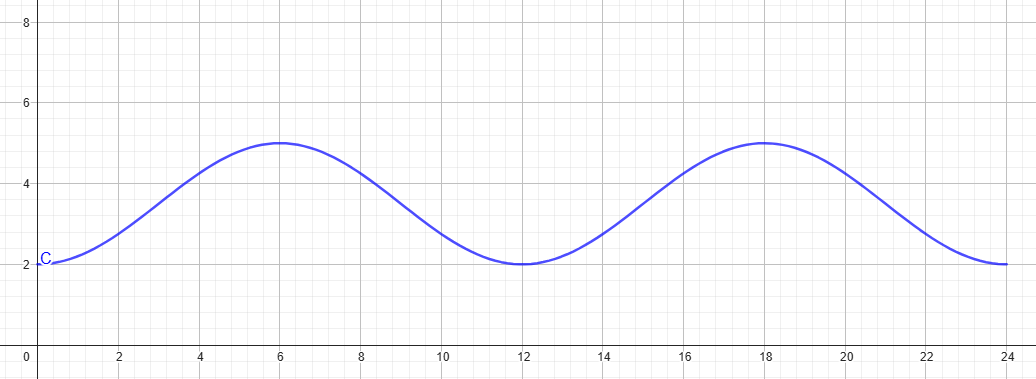
\includegraphics[width=0.9\linewidth]{image.png}
\end{figure}

\subsection{Calculá el consumo promedio de energía durante el día (de 0 a 24 h).}

$C_{promedio} = \frac{\int_{0}^{24} C(t)dt}{24} = \frac{84}{24} = \frac{7}{2}$\\

El consumo promedio fue de $\frac{7}{2}$ kW

\subsection{Usando el teorema del valor medio para integrales, determiná si existe algún instante del día en que el consumo instantáneo sea exactamente igual al consumo promedio. En caso afirmativo, hallá dicho instante.}

Sí, como la función $C(t)$ es continua en el intervalo $[0,24]$, entonces existirá un valor $c$ tal que la integral desde 0 hasta 24 de $C(t)$ sea igual a $f(c)(24 - 0)$

\begin{align*}
    C(t) &= C_{\text{promedio}} \\
    2 + 3\sin^2\left(\frac{\pi t}{12}\right) &= \frac{7}{2} \\
    3\sin^2\left(\frac{\pi t}{12}\right) &= \frac{3}{2} \\
    \sin^2\left(\frac{\pi t}{12}\right) &= \frac{1}{2} \\
    \frac{1 - \cos\left(\frac{\pi t}{6}\right)}{2} &= \frac{1}{2} \\
    1 - \cos\left(\frac{\pi t}{6}\right) &= 1 \\
    -\cos\left(\frac{\pi t}{6}\right) &= 0 \\
    \cos\left(\frac{\pi t}{6}\right) &= 0 \\
    \frac{\pi t}{6} &= \frac{\pi}{2} + k \pi \quad \implies \quad t = 3 + 6k \qquad k \in \mathbb{Z}
\end{align*}

Las horas a las que el consumo eléctrico es igual al promedio serán las 3, 9, 15 y 21.

\section{Costo mensual con variación progresiva}
\subsection{Calcula el precio diario correspondiente a los días 1 y 10, y determina la expresión de la progresión aritmética para ese tramo.}

En el día 1, el precio diario tiene un 10\% de descuento sobre los \$4,2/kWh, por lo que el precio para el día 1 será de \$3,78/kWh. \\

En el día 10, el precio diario será el normal, es decir \$4,2/kWh. \\

la progresión aritmética $a_n$ modela el precio por kWh para cada día $n$ entre los días 1 y 10

\begin{align*}
a_n &= a_1 + (n-1) \cdot d \\
a_{10} &= a_1 + 9 \cdot d\\
\frac{a_{10}-a_1}{9} &= d\\
\frac{4,2-3,78}{9} &= d \\
\boxed{0,0467} &= d
\end{align*}

{\centering{\boxed{a_n = 3,78 + (n-1) \cdot 0,0467}} \\}

\subsection{Calcula lo mismo para los días desde el 21 al 30.}

En el día 30, el precio diario será 15\% más caro que los \$4,2/kWh, por lo que el precio para el día 30 será de $4,2+(0,15\cdot4,2)=\$4,83/kWh$ \\

Entonces la diferencia total va a ser de $4,83 - 4,2 = 0,63$ que se reparte entre los 10 días.\\

$d = \frac{0,63}{10} = 0,063$ \\

Entonces el precio en el día 21 será de $\$4,2 + \$0,063 = \$4,263$ \\

Con un procedimiento análogo al de la parte anterior se llega a que la proogresión $b_n$ para los días 21 a 30 es la siguiente ($b_1$ equivale al día 21) \\

$b_n = 4,263+(n-1) \cdot 0,063$ 

\subsection{Usando fórmulas de progresiones aritméticas, calculá el costo mensual total para los 30 días.}

Para calcular el costo total de los 30 días hay que sumar los costos totales de los 3 grupos de 10 días. Como son progresiones aritméticas, la suma de los primeros n términos se calcula: \\

$S_n = \frac{(a_1 + a_n)}{2} \cdot n$ \\

Luego a  esta suma de los precios la multiplicamos por el consumo total de un día (84kW) \\

Costo para los días 1 al 10:

$P_1 = (\frac{3,78 + 4,2}{2} \cdot 10) \cdot 84  = 39,9 \cdot 84 = 3351,6$ \\

Costo para los días 11 al 20 (precio constante de $\$4,2/kWh$):

$P_2 = 4,2 \cdot 10 \cdot 84 = 3528 $\\

Costo para los días 21 al 30:

$P_3 = (\frac{4,263 + 4,83}{2} \cdot 10) \cdot 84  = 45,465 \cdot 84 = 3819,06$ \\


$P_{total} = P_1 + P_2 + P_3 = 10698,66$ \\

El consumo total es de $\$10698,66$

\section{Mejora de eficiencia}

\subsection{Calcula el nuevo consumo energético diario.}

$84 \cdot 0,80 = 67,2$

El nuevo consumo eléctrico diario es de $67,2 kWh$

\subsection{Determina en cuántos días la inversión se amortiza considerando el ahorro energético diario.}

El ahorro energético diario es de $84kWh-\$67,2kWh = 16,8kWh$ \\

El precio medio del kWh en el período de 30 días va a ser:
$\frac{P_{total}}{84\cdot 30} = \frac{\$10698,66}{2520} = \$4,2455$ \\

Por lo tanto, el ahorro monetario diario va a ser de: \\

$16,8 \cdot 4,2455 = \$71,3244$ \\

Como la inversión fue de $\$150.000$ \\

$Dias = \frac{150.000}{71,3244} = 2103$ \\

Por lo tanto, la inversión queda amortizada en 2103 días.

\subsection{Representa con una sucesión el ahorro acumulado después de n días, y determina si converge o no.}

$A_n = 71,3244 \cdot n$

Como el límite cuando $n$ tiende a $+\infty$ de $A_n$ es $+\infty$, la sucesión no converge.

\section{Parte 4: Pérdida acumulada por ineficiencia}

\subsection{}
$F_n = (\frac{5}{n})^2$

\[ \sum_{n=1}^{\infty}F_{n} = \sum_{n=1}^{\infty}\left(\frac{5}{n}\right)^{2} = 25 \sum_{n=1}^{\infty}\frac{1}{n^{2}} \]

Según los criterios de convergencia para las series de tipo armónica generalizada, la serie converge porque $p=2$ y $2 > 1$

\subsection{ Calculá la pérdida total de energía acumulada en los primeros 30 días. ¿Cómo se compara con el consumo diario total?}

Para calcular la fuga acumulada de energía en los primeros 30 días hacemos la sumatoria desde n=1 hasta n=30

\[ S_{30} = \sum_{n=1}^{30}\left(\frac{5}{n}\right)^{2} = 25 \sum_{n=1}^{30}\frac{1}{n^{2}} \approx 25 \times 1,61226 \approx 40,31 \text{ kWh} \] \\

La fuga total de energía es de aproximadamente $40kWh$ que es aproximadamentet la mitad del consumo diario de energía.

\subsection{Si cada kWh cuesta 4,2 pesos, estimá el costo económico de esa pérdida.}

$Costo = 40,31 \cdot 4,2 = 169,30$ \\

La pérdida económica es de $\$169,302$

\subsection{Compará ese valor con el ahorro mensual generado por los paneles solares (ver Parte 3). ¿Cuál de los dos tiene mayor impacto económico?}

Como el ahorro diario de los paneles solares era de $\$71, 3244$, el ahorro mensual de los paneles será de $\$71,3244 \cdot 30 = \$2139,732$ \\

O sea que el ahorro económico de los paneles tiene un impacto economico mucho mayor que la fuga de energía.
\end{document}
